\documentclass[a4paper]{article}

\usepackage[fontset=fandol]{ctex}
\usepackage{amsmath, amssymb}
\usepackage{graphicx}
\usepackage[margin=2.3cm]{geometry}
\usepackage[most]{tcolorbox}
\usepackage{listings}
\usepackage{hyperref}
\usepackage{booktabs}
\usepackage{float}
\usepackage{xcolor}

\lstset{
    language=Python,
    basicstyle=\ttfamily\small,
    keywordstyle=\color{blue},
    stringstyle=\color{red!60!black},
    commentstyle=\color{green!50!black},
    breaklines=true,
    frame=single,
    numbers=left,
    numberstyle=\tiny\color{gray}
}

\newtcolorbox{knowledgebox}[1]{
    enhanced,
    colback=blue!5!white,
    colframe=blue!70!black,
    colbacktitle=blue!70!black,
    coltitle=white,
    fonttitle=\bfseries,
    title=#1,
    sharp corners
}

\newtcolorbox{importantbox}[1]{
    enhanced,
    colback=yellow!10!white,
    colframe=yellow!70!black,
    colbacktitle=yellow!70!black,
    coltitle=black,
    fonttitle=\bfseries,
    title=#1,
    sharp corners
}

\newtcolorbox{warningbox}[1]{
    enhanced,
    colback=red!5!white,
    colframe=red!70!black,
    colbacktitle=red!70!black,
    coltitle=white,
    fonttitle=\bfseries,
    title=#1,
    sharp corners
}

\begin{document}

\begin{titlepage}
\centering
{\Large 课程讲义\par}
\vspace{1.2cm}
{\huge\bfseries Inference-Time Techniques for LLM Reasoning\par}
\vspace{0.6cm}
{\Large CS294/194-280: Advanced Large Language Model Agents\par}
\vspace{0.4cm}
{\large Xinyun Chen, Google DeepMind\par}
\vspace{0.4cm}
{\large 中文教材化讲义 / Codex Harness Build\par}
\vspace{0.8cm}
\includegraphics[width=0.84\textwidth,height=0.38\textheight,keepaspectratio]{cover.jpg}\par
\vfill
\begin{tcolorbox}[width=0.92\textwidth,colback=black!2!white,colframe=black!60,sharp corners]
\textbf{课程页}：\href{https://rdi.berkeley.edu/adv-llm-agents/sp25}{https://rdi.berkeley.edu/adv-llm-agents/sp25}\par
\textbf{录播}：\href{https://www.youtube.com/live/g0Dwtf3BH-0}{https://www.youtube.com/live/g0Dwtf3BH-0}\par
\textbf{主 slides}：\href{https://rdi.berkeley.edu/adv-llm-agents/slides/inference_time_techniques_lecture_sp25.pdf}{inference\_time\_techniques\_lecture\_sp25.pdf}\par
\textbf{导入 slides}：\href{https://rdi.berkeley.edu/adv-llm-agents/slides/llm-agents-berkeley-intro-sp25.pdf}{llm\_agents\_berkeley\_intro\_sp25.pdf}\par
\textbf{补充 readings}：OPRO / LLMs Cannot Self-Correct Reasoning Yet / Self-Debugging
\end{tcolorbox}
\end{titlepage}

\tableofcontents
\newpage

\section{本讲学习目标}

本讲是整门课的技术起点。它关心的问题不是“如何重新训练一个更强的 base model”，而是：在\textbf{推理时计算（inference-time computation）}固定可控的前提下，如何把同一个语言模型变成更会推理、更会搜索、更会自我修订的系统。读完本讲后，读者应当能够回答以下问题：

\begin{itemize}
\item 为什么 2024--2025 年的 reasoning models 让 \emph{test-time compute} 重新成为核心设计变量。
\item Standard prompting、Few-shot Chain-of-Thought、Zero-shot CoT、Analogical Prompting 分别解决什么问题，各自失败在哪里。
\item 为什么可以把 prompt engineering 改写成一个显式的优化、搜索或结构发现过程。
\item Self-Consistency、Verifier、Tree of Thoughts、Self-Debugging 的共同本质是什么，它们彼此如何互补。
\item 为什么没有可靠外部反馈时，self-correction 往往并不会自动成功。
\item 在预算有限时，如何在模型规模、并行采样宽度、串行修正深度之间做取舍。
\end{itemize}

\section{背景与问题设置}

\subsection{从 LLM 到 LLM agent：为什么课一开始就讲 inference-time techniques}

这门课不是把 LLM 当成单次文本生成器，而是把它放进一个\textbf{agent-environment 闭环}中：模型需要感知环境，进行推理与规划，调用工具、使用记忆、执行动作，再根据反馈继续调整策略。导入 slides 的第一张核心图正是这个闭环。

\begin{figure}[H]
\centering
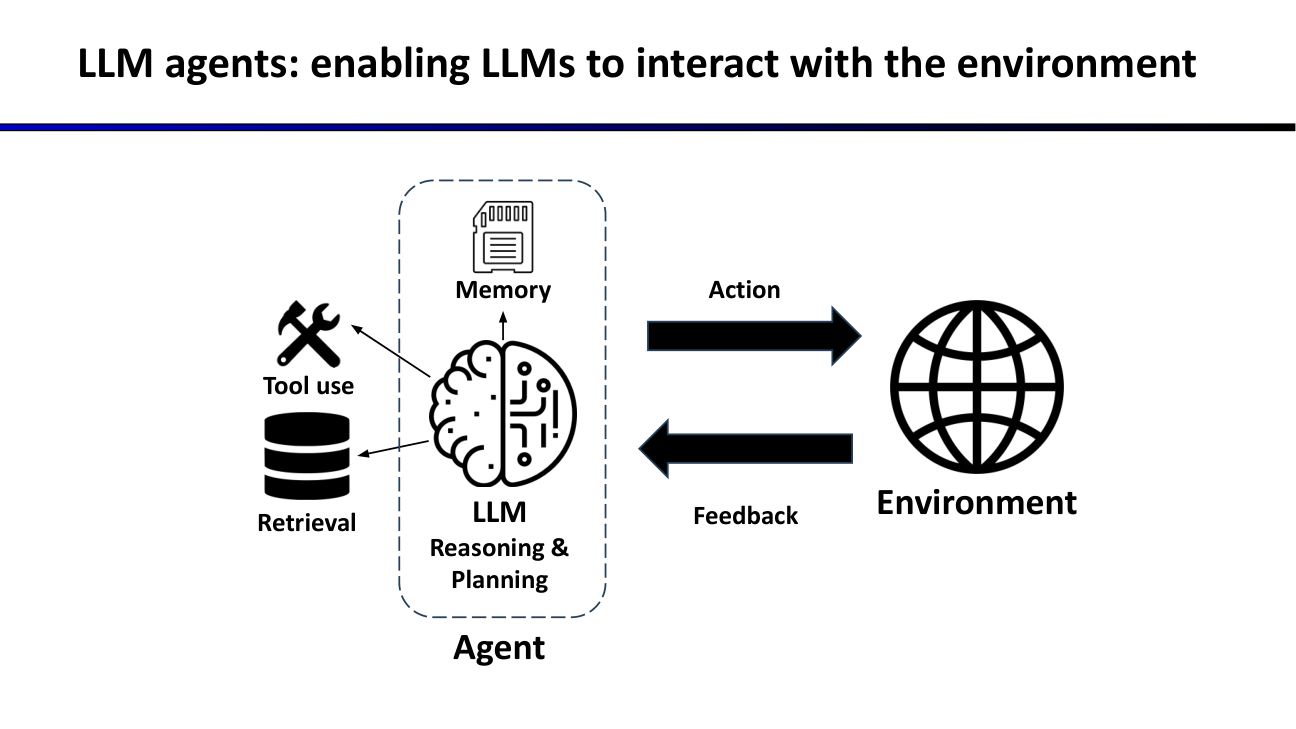
\includegraphics[width=0.84\textwidth]{figures/lec01_fig_001.png}
\caption{LLM agent 与 environment 的闭环：推理、工具、记忆、行动和反馈共同构成 agent workflow。}
\end{figure}

如果只把模型当成“输入问题，吐出答案”的函数，那么我们几乎只能从参数规模、预训练数据和后训练流程上寻求性能提升。但一旦把模型视为 agent，问题就变成：同一个模型是否可以通过更好的\textbf{推理路径组织、搜索策略、外部评价器和反馈循环}，在不改权重或少改权重的情况下做得更好？

这就是本讲的出发点。课程导入页给出了 2024--2025 年 reasoning models 的发展节点，例如 OpenAI o1/o3、Gemini 2.0 Flash Thinking、DeepSeek-R1 等，这些系统共同强调了一个事实：\textbf{不是只有训练时算力重要，推理时如何分配算力也变成了性能上限的重要决定因素。}

\begin{figure}[H]
\centering
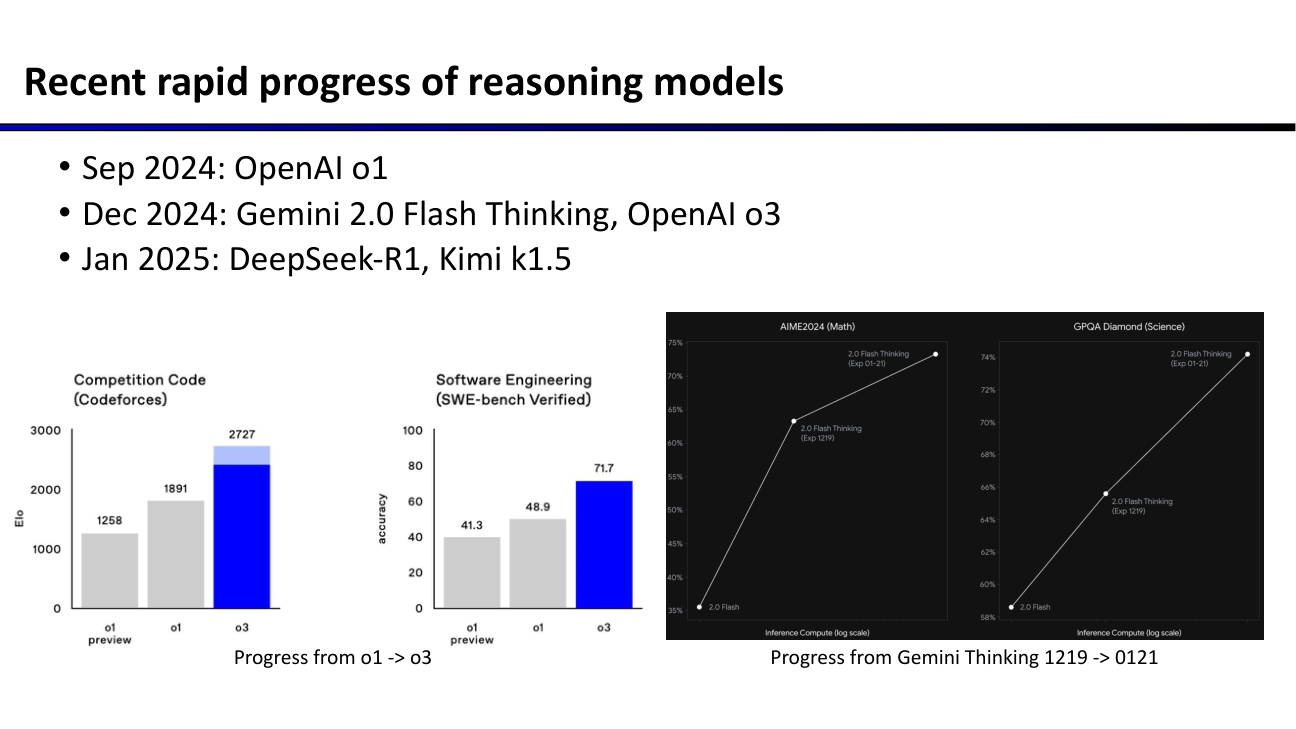
\includegraphics[width=0.78\textwidth]{figures/lec01_fig_002.png}
\caption{导入 slides 中的 reasoning model 时间线。课程把它放在第一讲开头，表明 test-time reasoning 已经从技巧变成系统设计主线。}
\end{figure}

\subsection{问题重述：把更多计算花在“想法质量”上}

主 slides 很早就给出一个关键观察：\textbf{随着更多 inference-time compute 的投入，性能通常会上升，但成本也会显著上升。} 这意味着我们真正优化的不是“能不能多想”，而是“多出来的计算应该花在哪种推理结构上才最值”。

\begin{figure}[H]
\centering
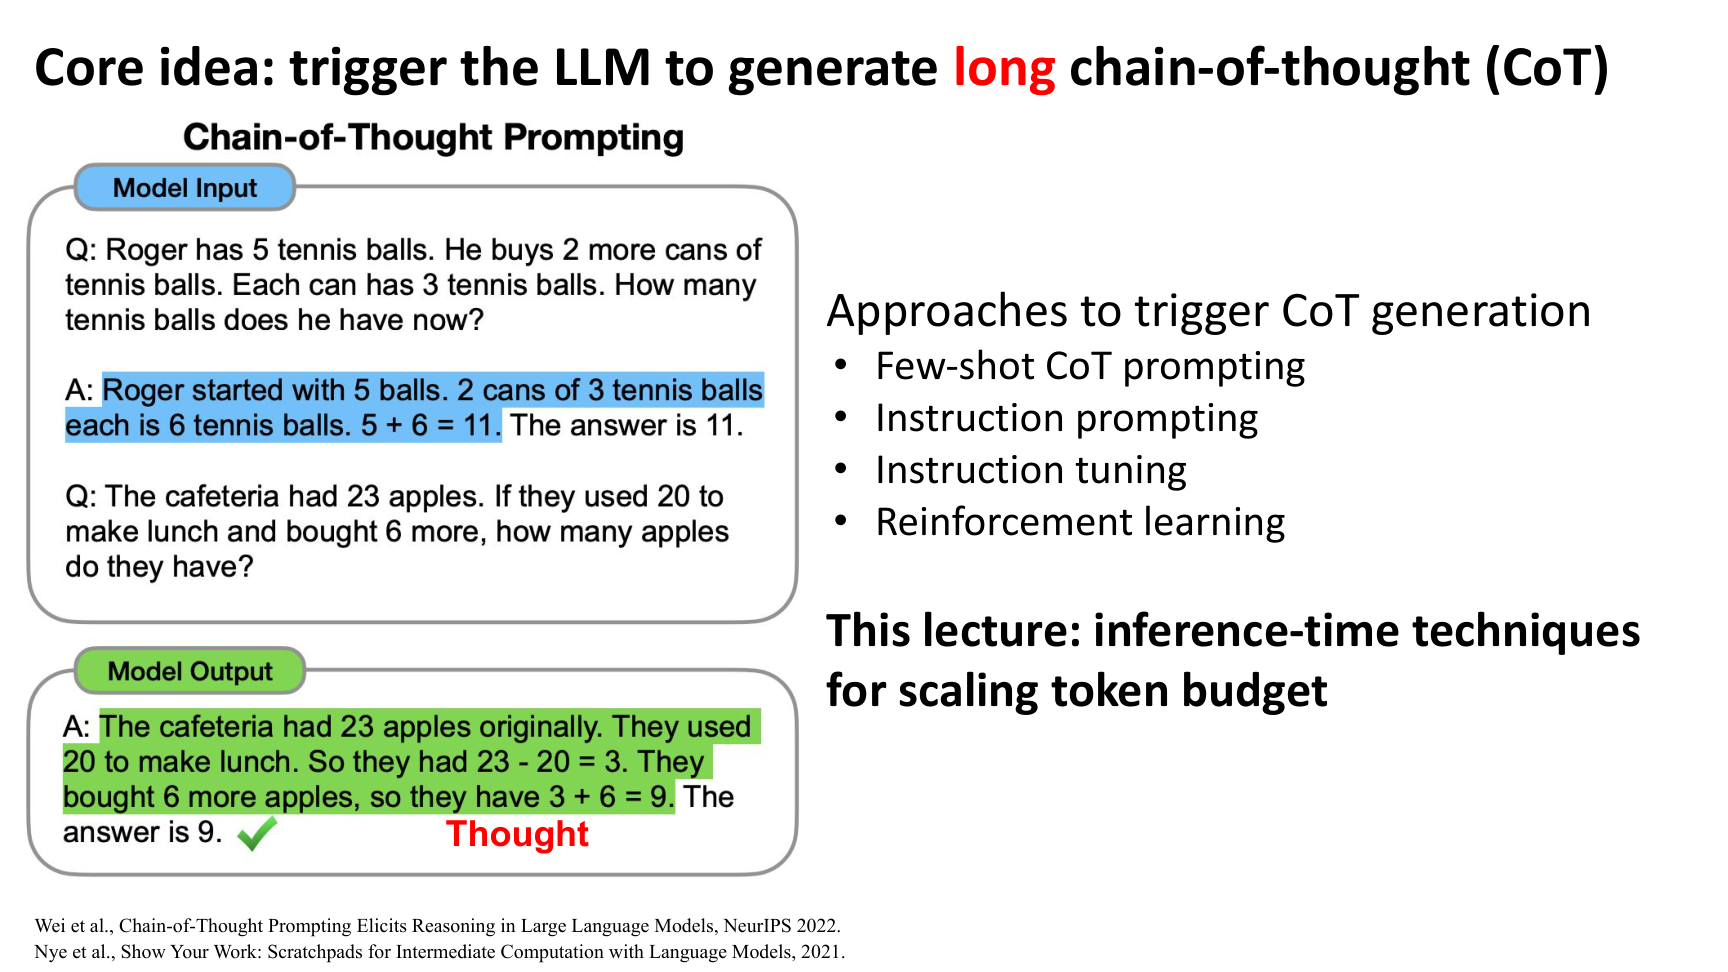
\includegraphics[width=0.82\textwidth]{figures/lec01_fig_003.png}
\caption{本讲的总纲：让模型在推理时产生更长、更丰富、可验证或可搜索的 reasoning trace。}
\end{figure}

朴素做法是直接要求模型“想一想”，但这只是把更多 token 花在单条推理轨迹上。更系统的做法包括：

\begin{itemize}
\item 在\textbf{单轨路径}上改进提示结构，例如 CoT、Analogical Prompting、Least-to-Most。
\item 在\textbf{多路径宽搜索}上做聚合，例如 Self-Consistency。
\item 在\textbf{路径评分}上引入 verifier 或 reward model。
\item 在\textbf{部分解空间}上做搜索，例如 Tree of Thoughts。
\item 在\textbf{迭代修订}上利用外部信号，例如 Self-Debugging。
\end{itemize}

\begin{knowledgebox}{本讲的统一视角}
可以把本讲的各种方法看成同一类设计空间中的不同点：它们都在试图改善“候选推理轨迹的生成方式”和“候选轨迹的选择方式”。前者决定我们探索什么，后者决定我们保留什么。
\end{knowledgebox}

\subsection{核心概念与术语}

\begin{itemize}
\item \textbf{推理时计算（inference-time computation）}：部署后在一次任务求解中额外花费的计算资源，如更长的 CoT、更宽的采样、更深的修正循环、更强的 verifier。
\item \textbf{单轨推理（single-path reasoning）}：模型只生成一条主要思路，然后直接产出答案。
\item \textbf{宽搜索（breadth at inference time）}：并行生成多条候选思路，再聚合或筛选。
\item \textbf{深搜索 / 迭代修订（depth / iterative refinement）}：对同一问题进行多轮分析、反思、修正。
\item \textbf{Verifier}：对完整答案或中间步骤打分的评价器。Lecture 中区分了 outcome reward model（ORM）与 process reward model（PRM）。
\item \textbf{外部反馈（external feedback）}：来自测试用例、执行 trace、oracle、环境奖励、形式验证器等独立于模型自说自话的信号。
\end{itemize}

\section{主体讲解：从单轨推理到搜索与自改进}

\subsection{Standard Prompting、Few-shot CoT 与 Zero-shot CoT}

Standard prompting 的基本范式是：把任务描述、输入和输出格式告诉模型，期待它一步给出最终答案。它的最大问题不是“模型不会说话”，而是\textbf{没有显式分配任何 token 预算给中间推理}。当任务只需要表层模式匹配时，这种范式足够；一旦任务包含组合推理、算术、多步逻辑或需要结构化中间状态，模型很容易在一跳里出错。

Few-shot Chain-of-Thought（CoT）做了一个关键改变：示例不再只给出 \emph{input-output} 对，而是把\emph{中间思考过程}也暴露出来。这样模型学到的就不是“答案形式”，而是“如何把问题展开成一串中间步骤”。主 slides 强调 CoT 的增益会随着模型规模上升而增强，这说明 CoT 并不是简单模板 trick，而是在更大模型中激活了更强的隐式推理能力。

Zero-shot CoT 更进一步：它不再依赖人工构造演示样例，而是用类似 “Let's think step by step” 的指令触发模型展开推理。其重要意义在于，它证明了很多 reasoning gain 来自\textbf{解码时轨迹展开}，而不完全来自示例记忆。

\begin{figure}[H]
\centering
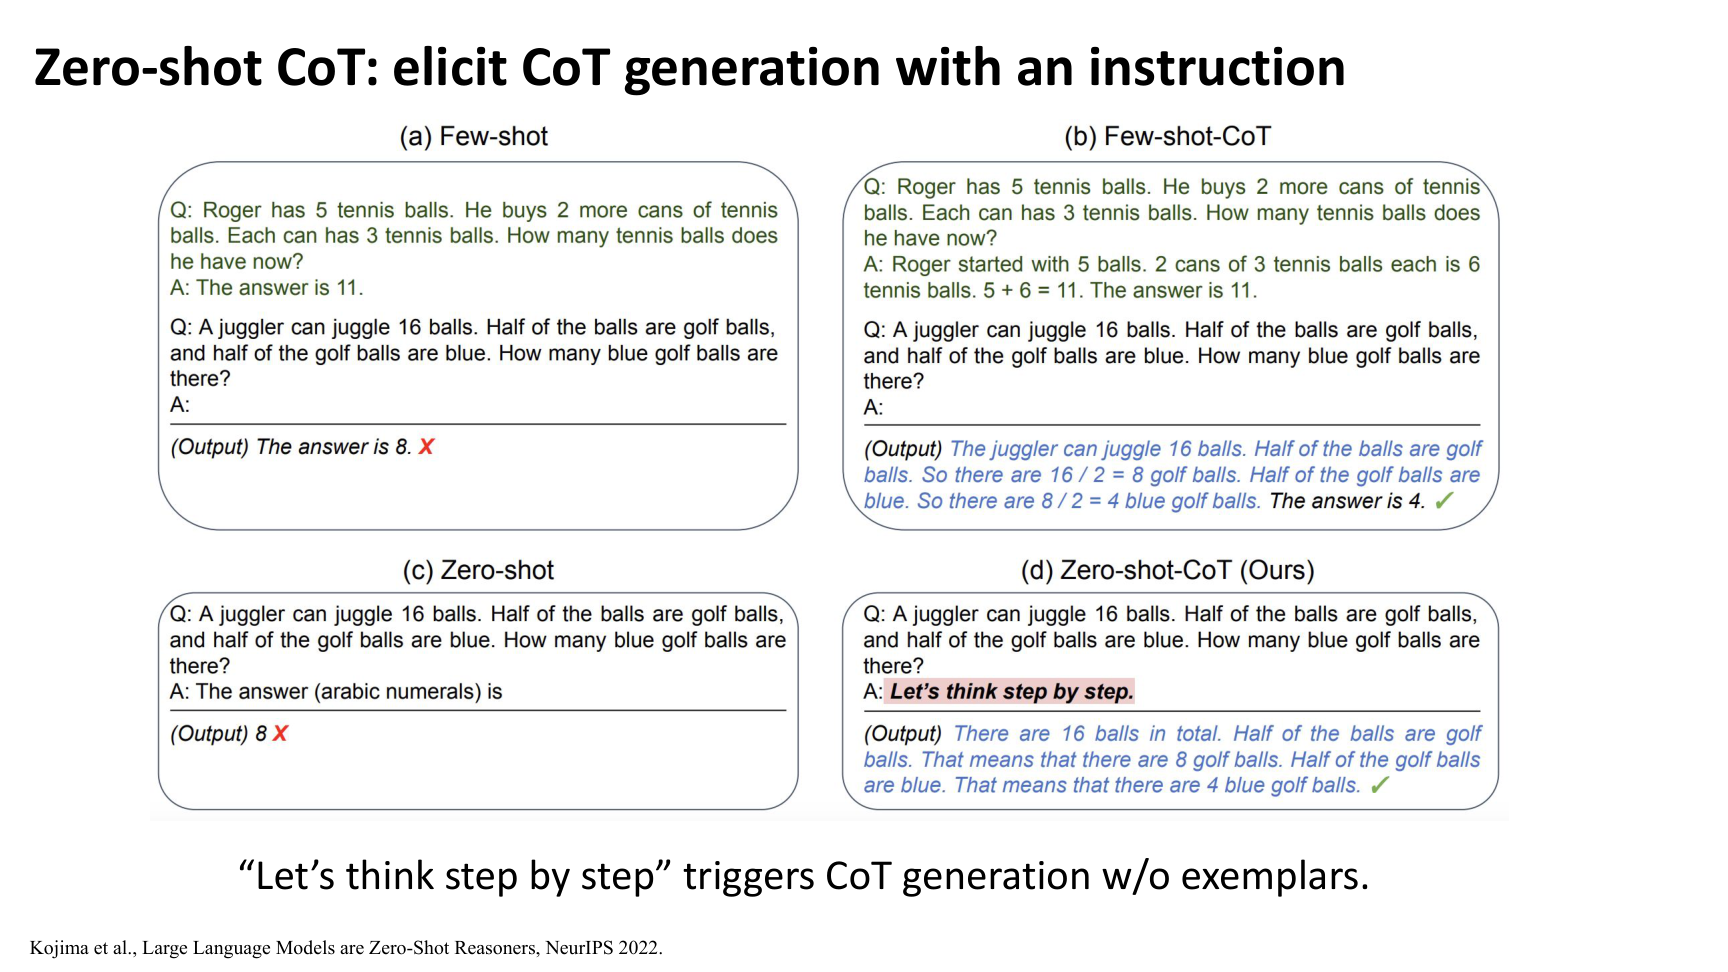
\includegraphics[width=0.74\textwidth]{figures/lec01_fig_004.png}
\caption{Zero-shot CoT 的典型触发方式：通过一句显式指令，把模型从“直接回答模式”切换到“先推理后回答模式”。}
\end{figure}

\begin{importantbox}{为什么朴素方法不够}
如果没有显式推理轨迹，模型的错误往往只能在最终答案层面观察，无法知道它究竟是知识缺失、局部算错、结构没展开，还是早期步骤就走偏了。CoT 的价值首先是把“错误位置”暴露出来。
\end{importantbox}

\paragraph{小例子}
在算术文字题里，standard prompting 直接要求模型输出答案，常常会跳过单位换算或中间求和。Few-shot CoT 则展示“先找数值、再列式、再求解”的轨迹；Zero-shot CoT 则用一句指令让模型自动展开类似轨迹。三者的差别，本质上是\textbf{是否把一部分 token budget 强制分配给中间状态}。

\paragraph{边界条件}
CoT 并不保证正确。若模型本身不会该任务，或生成的中间步骤只是看起来像推理而并不受真实状态约束，那么更长的 CoT 只会产生\textbf{更长的错误解释}。

\subsection{Analogical Prompting：先回忆相似例子，再解当前题}

Analogical Prompting 把问题推进了一步：与其直接解当前问题，不如先让模型回忆与当前任务相似的 exemplars，再根据这些 exemplars 去求解。这一做法的直觉是，很多复杂问题的难点不是不会算，而是\textbf{没有找到合适的解题模板}。通过先回忆相似案例，可以降低模型检索和组织解法结构的负担。

\begin{figure}[H]
\centering
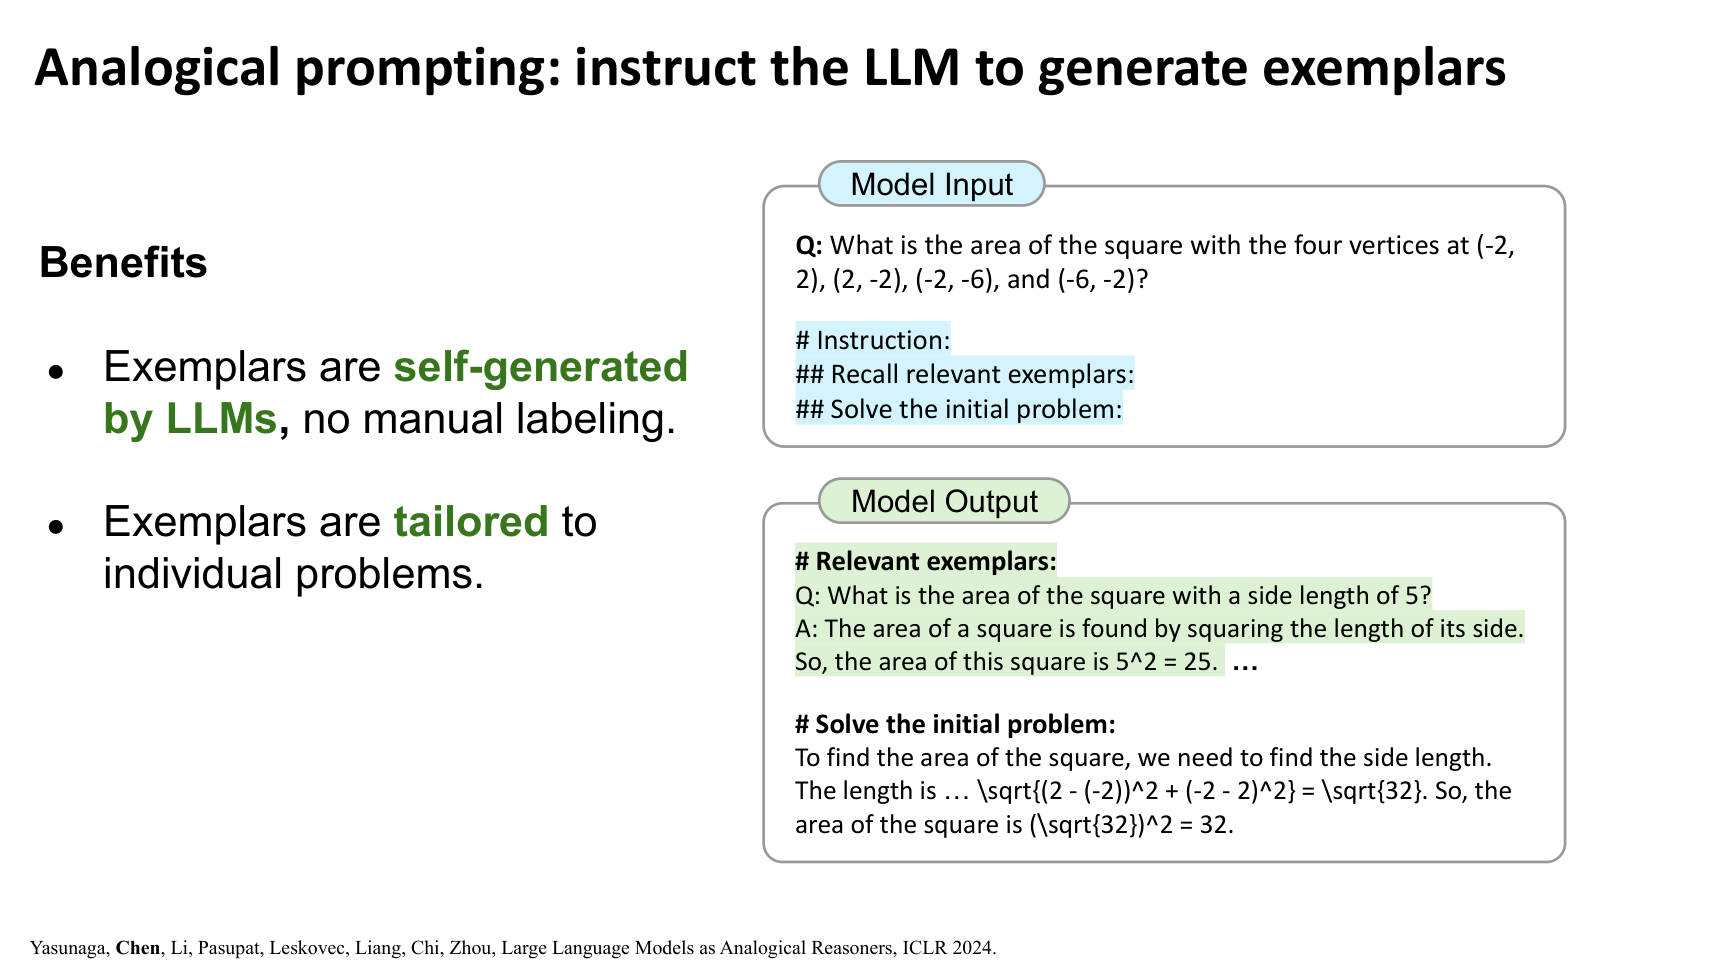
\includegraphics[width=0.74\textwidth]{figures/lec01_fig_005.png}
\caption{Analogical Prompting 的两阶段结构：先检索/生成相关 exemplars，再利用这些 exemplars 解当前问题。}
\end{figure}

这类方法解决的不是“计算能力不够”，而是“解题起点不对”。当模型面对几何题、数学题或推理谜题时，往往最难的是辨认当前题型与哪一类已有解法最接近。Analogical Prompting 通过让模型先回忆，再求解，相当于在 inference time 做一次轻量的\textbf{结构检索}。

\begin{lstlisting}
Instruction:
1. Recall relevant exemplars for the current task.
2. Solve the initial problem using the recalled exemplars.
\end{lstlisting}

上面这段伪代码并不复杂，但它体现的机制很关键：它把“回忆解法模板”和“执行该模板”分成两个阶段。Lecture 中还展示了强模型比弱模型更像 analogical reasoner 的结果，这说明这种方法并非对所有模型都同样有效。更强的模型拥有更稳定的内隐 pattern library，因此更能从自生成 exemplars 中受益。

\paragraph{失败模式}
\begin{itemize}
\item 如果模型回忆的 exemplars 本身就是错的，那么后续推理会被系统性带偏。
\item 如果任务需要精确的外部状态，而 exemplars 只是表面相似，那么类比会制造虚假的信心。
\item 若模型规模偏小，回忆阶段可能退化成空泛 paraphrase，反而浪费预算。
\end{itemize}

\subsection{把 Prompt Engineering 变成优化：OPRO、Least-to-Most 与 Self-Discover}

\subsubsection{OPRO：LLM 既是求解器，也是优化器}

Lecture 在这一段做了一个非常重要的转向：不再把 prompt 视为静态手工产物，而是把它看成可以被搜索、修改、评价的对象。OPRO（\emph{Large Language Models as Optimizers}）就是这一思想的代表。

\begin{figure}[H]
\centering
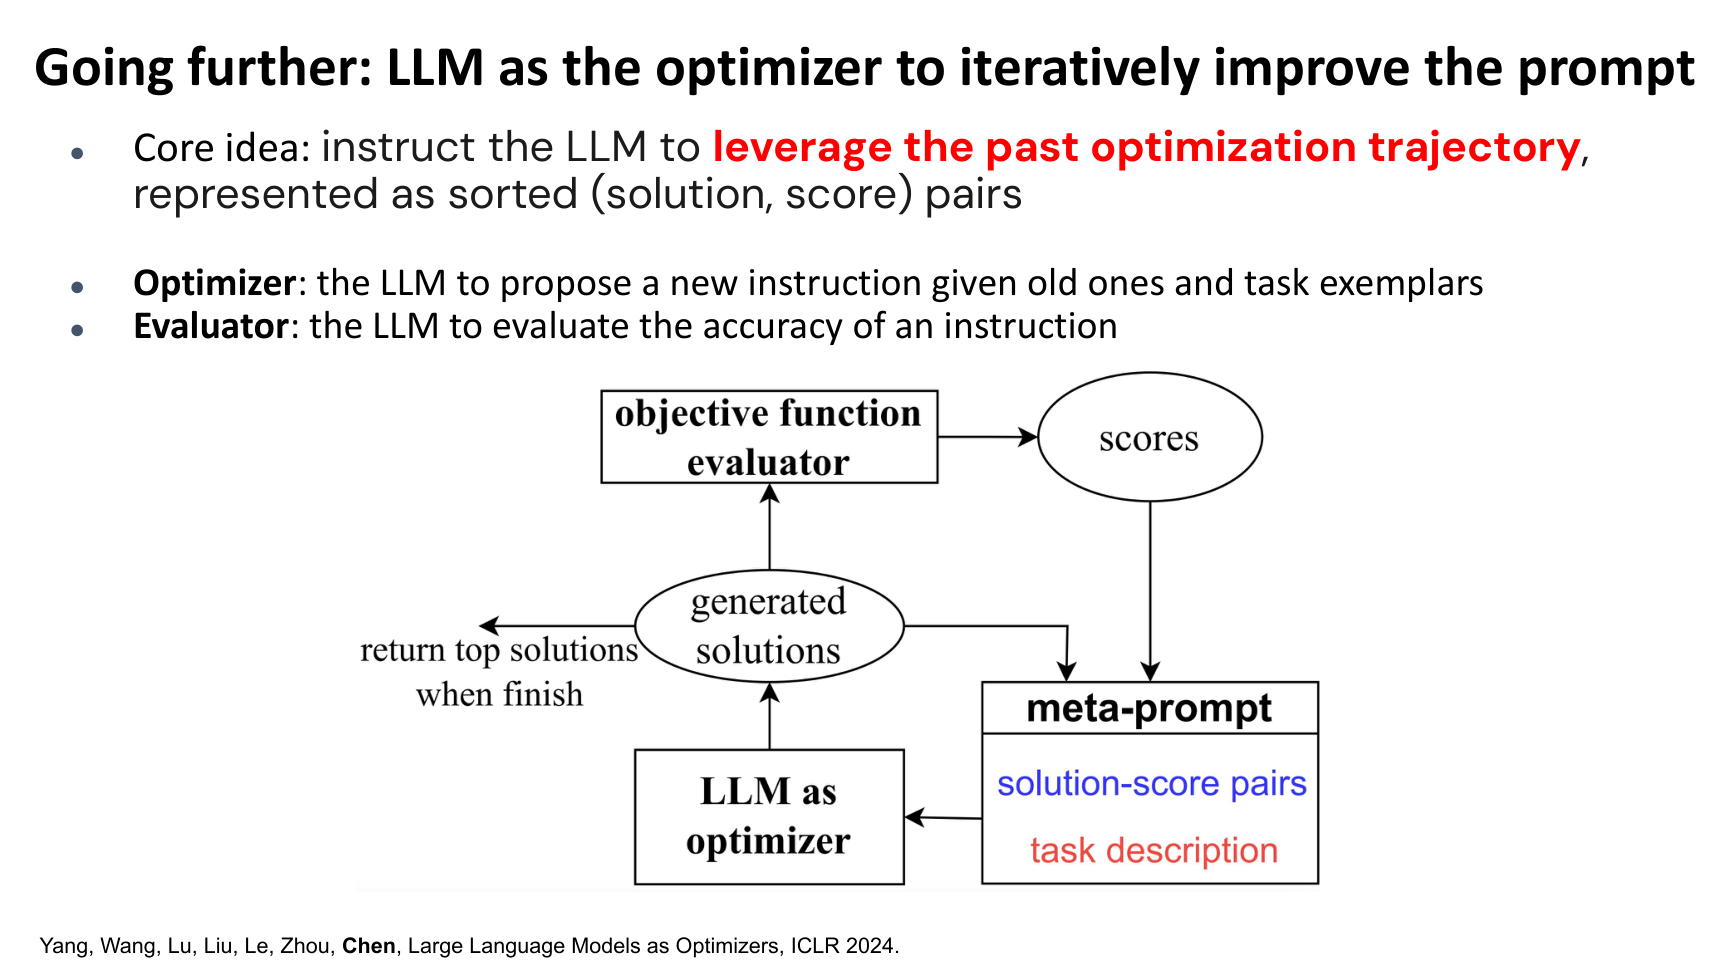
\includegraphics[width=0.78\textwidth]{figures/lec01_fig_006.png}
\caption{OPRO 的优化循环：维护候选 instruction 及其得分历史，让 LLM 根据历史继续提出新候选。}
\end{figure}

形式化地说，OPRO 可以被写成：
\[
x_{t+1} \sim \operatorname{LLM}\left(\{(x_i, s_i)\}_{i=1}^{t}, \mathcal{E}\right)
\]
其中，$x_i$ 是第 $i$ 轮已有的 instruction 或候选解，$s_i$ 是该候选在验证集上的得分，$\mathcal{E}$ 表示任务 exemplars 或任务说明，$x_{t+1}$ 则是语言模型在观察优化历史后提出的新候选。

这条公式背后的直觉是：\textbf{只要我们能定义一个可观测分数，语言模型就可以把过去的尝试轨迹当成优化上下文，继续提出更好的文本候选。} 这使 prompt engineering 从“工程师灵感”转变成“迭代搜索”。

\begin{lstlisting}
Initialize instruction x0
for t in 0..T-1:
    score xt on a validation set
    append (xt, score) to the optimization history
    ask the LLM to propose xt+1 from the sorted history
\end{lstlisting}

\paragraph{为什么朴素 prompt tweaking 不够}
人工改 prompt 的主要问题在于不可系统扩展：你很难可靠记住哪些变体试过、为什么失败、下一轮应沿哪个方向修改。OPRO 则显式维护历史与分数，把优化路径变成推理对象。

\paragraph{Reading 连接}
\emph{Large Language Models as Optimizers} 证明了，在 GSM8K、BBH 等 prompt optimization 任务中，LLM 可以仅凭优化历史提出越来越好的 instruction。它的重要性不只在于“prompt 能被优化”，而在于它把\textbf{语言模型自身当成优化器}，打开了 inference-time search over prompts 这一方向。

\subsubsection{Least-to-Most 与 Self-Discover：结构本身也可以被推理时生成}

Least-to-Most Prompting 的核心思想是：复杂任务之所以难，不是因为最终答案太复杂，而是因为它缺乏正确的\textbf{子问题分解顺序}。因此先求简单子问题，再把结果递交给更难的子问题，就能在 compositional generalization 场景中获得更稳定的性能。

它解决的问题是：单次 CoT 虽然展开了思路，但\textbf{不一定找到正确的分解层次}。Least-to-Most 让模型先学会“拆”，再学会“合”。

Self-Discover 则把这一思想继续推进：既然不同任务适合不同 reasoning structure，那么不应人为固定一套 prompt template，而应让模型自己为当前任务\textbf{组装最合适的 reasoning structure}。

\begin{figure}[H]
\centering
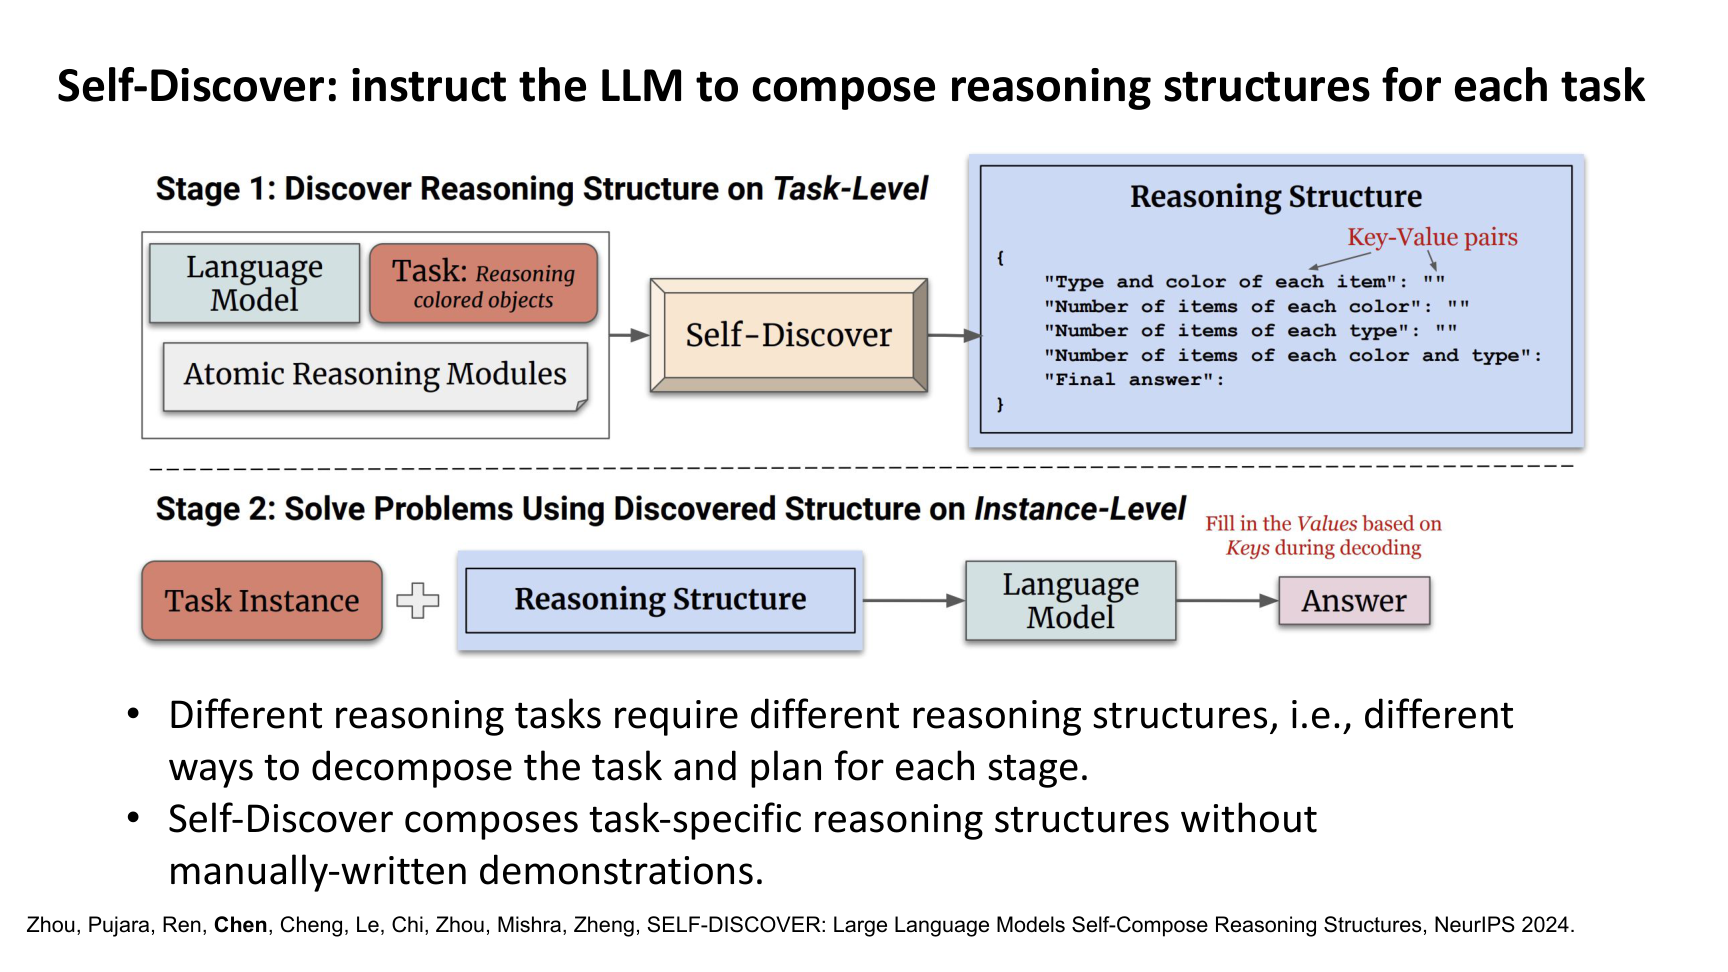
\includegraphics[width=0.72\textwidth]{figures/lec01_fig_007.png}
\caption{Self-Discover 的关键点：让模型按任务需要组合 reasoning modules，而不是固定使用某一种提示模板。}
\end{figure}

\begin{warningbox}{关键 caveat}
这类方法都依赖一个前提：模型不仅会执行某个推理结构，还大致知道\emph{什么时候}该用哪种结构。若模型对任务类型的判断不稳，自动结构发现可能退化成不必要的复杂 prompt。
\end{warningbox}

\subsection{宽搜索：Self-Consistency、执行一致性与 Universal Self-Consistency}

\subsubsection{Self-Consistency：不是只找一条路，而是比较多条路的终点}

Self-Consistency 的思想非常朴素但影响极大：不要只依赖一条采样到的 reasoning path，而是采样多条不同思路，然后只在最终答案层做聚合。它的形式化写法可以写成：
\[
\hat{y} = \arg\max_{y} \sum_{i=1}^{N} \mathbf{1}[\operatorname{extract}(a_i)=y]
\]
其中，$\hat{y}$ 是最终聚合答案，$a_i$ 是第 $i$ 条 sampled reasoning path 的完整输出，$\operatorname{extract}(a_i)$ 表示从该输出中抽取的最终答案，$N$ 是采样到的候选路径数量。

\begin{figure}[H]
\centering
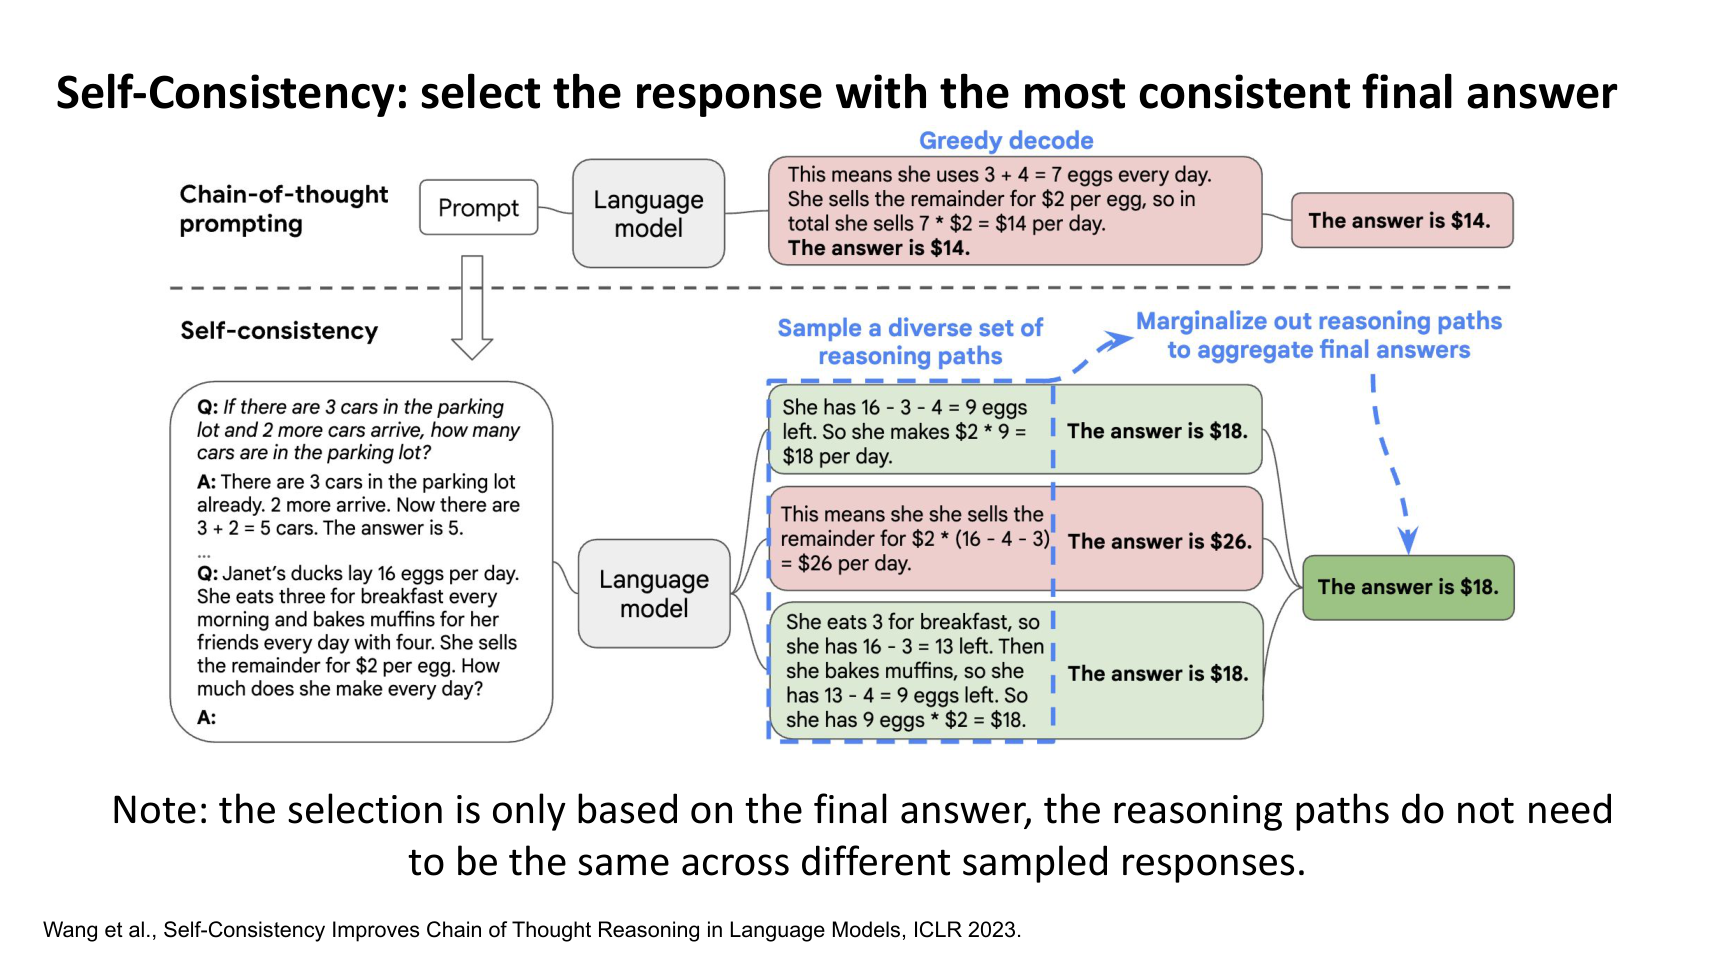
\includegraphics[width=0.73\textwidth]{figures/lec01_fig_008.png}
\caption{Self-Consistency 的直觉：不是押注单一路径，而是对多条 reasoning path 的终点做投票。}
\end{figure}

它的核心机制不是“多数人总是对的”，而是：如果问题允许多种正确推理路径，那么\textbf{正确答案往往会从多条独立路径中收敛出来}，而偶然错误则更分散。Lecture 进一步展示了：更多 samples 往往带来更高性能，但前提是采样要有多样性；若所有路径都高度相似，那么宽搜索没有真正增加探索。

\begin{figure}[H]
\centering
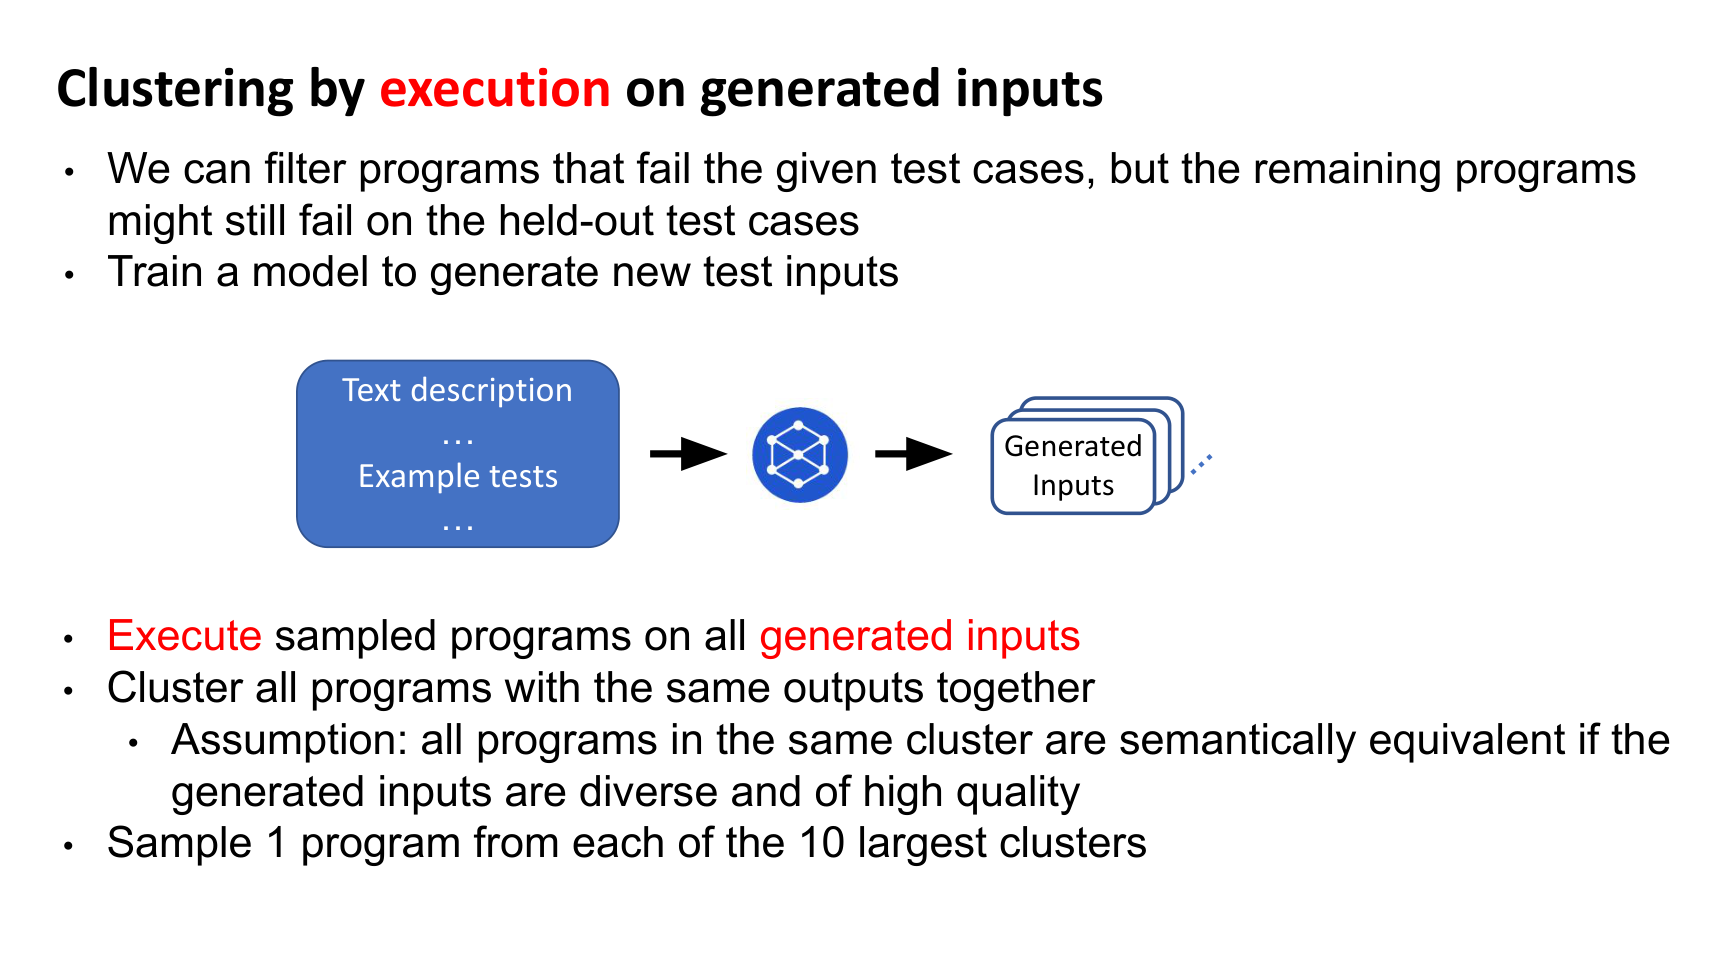
\includegraphics[width=0.73\textwidth]{figures/lec01_fig_009.png}
\caption{代码任务中的执行一致性。AlphaCode 类方法利用测试输入上的执行结果做聚类，比纯文本表面一致性更接近任务目标。}
\end{figure}

\paragraph{为什么 beam search 不等价}
Beam search 倾向于保留局部概率高的前缀，但 reasoning 任务中的正确路径不一定在早期 token 上最高概率。Self-Consistency 则通过\textbf{末端答案聚合}绕开了这一偏差。

\paragraph{代码任务中的更强信号}
对于代码生成，仅仅比较文本相似性不够。Lecture 用 AlphaCode 风格的结果说明，若能够根据程序在测试输入上的执行结果进行聚类或筛选，就能得到比文本一致性更强的选择信号。这也是“为何代码任务常常是自改进方法天然试验场”的重要原因：\textbf{它们拥有外部可执行的评价器。}

\subsubsection{Universal Self-Consistency}

Lecture 还提到 Universal Self-Consistency，其动机是：并不是所有任务都能轻松抽取一个明确的终点答案。于是可以让模型本身承担“比较候选 reasoning traces 是否一致”的工作。它把一致性判断从手工设计的答案抽取器扩展到了更一般的生成场景。

这类方法的好处是适用面更广，但缺点也明显：一旦让模型自己做一致性判断，就再次回到了“评价器是否可靠”的问题。若 LLM judge 本身不稳定，Universal Self-Consistency 只是把问题从生成端挪到了选择端。

\subsection{评分器与部分解搜索：Verifier、PRM/ORM 与 Tree of Thoughts}

\subsubsection{Verifier：Outcome-level 和 Process-level 的区别}

Self-Consistency 已经引入“生成多条候选再选”的思路，但它仍然只在终点上比较答案。Lecture 接着提出 verifier：如果我们能训练或设计一个更强的评分函数，它就不必等完整答案生成完毕才介入。

\begin{figure}[H]
\centering
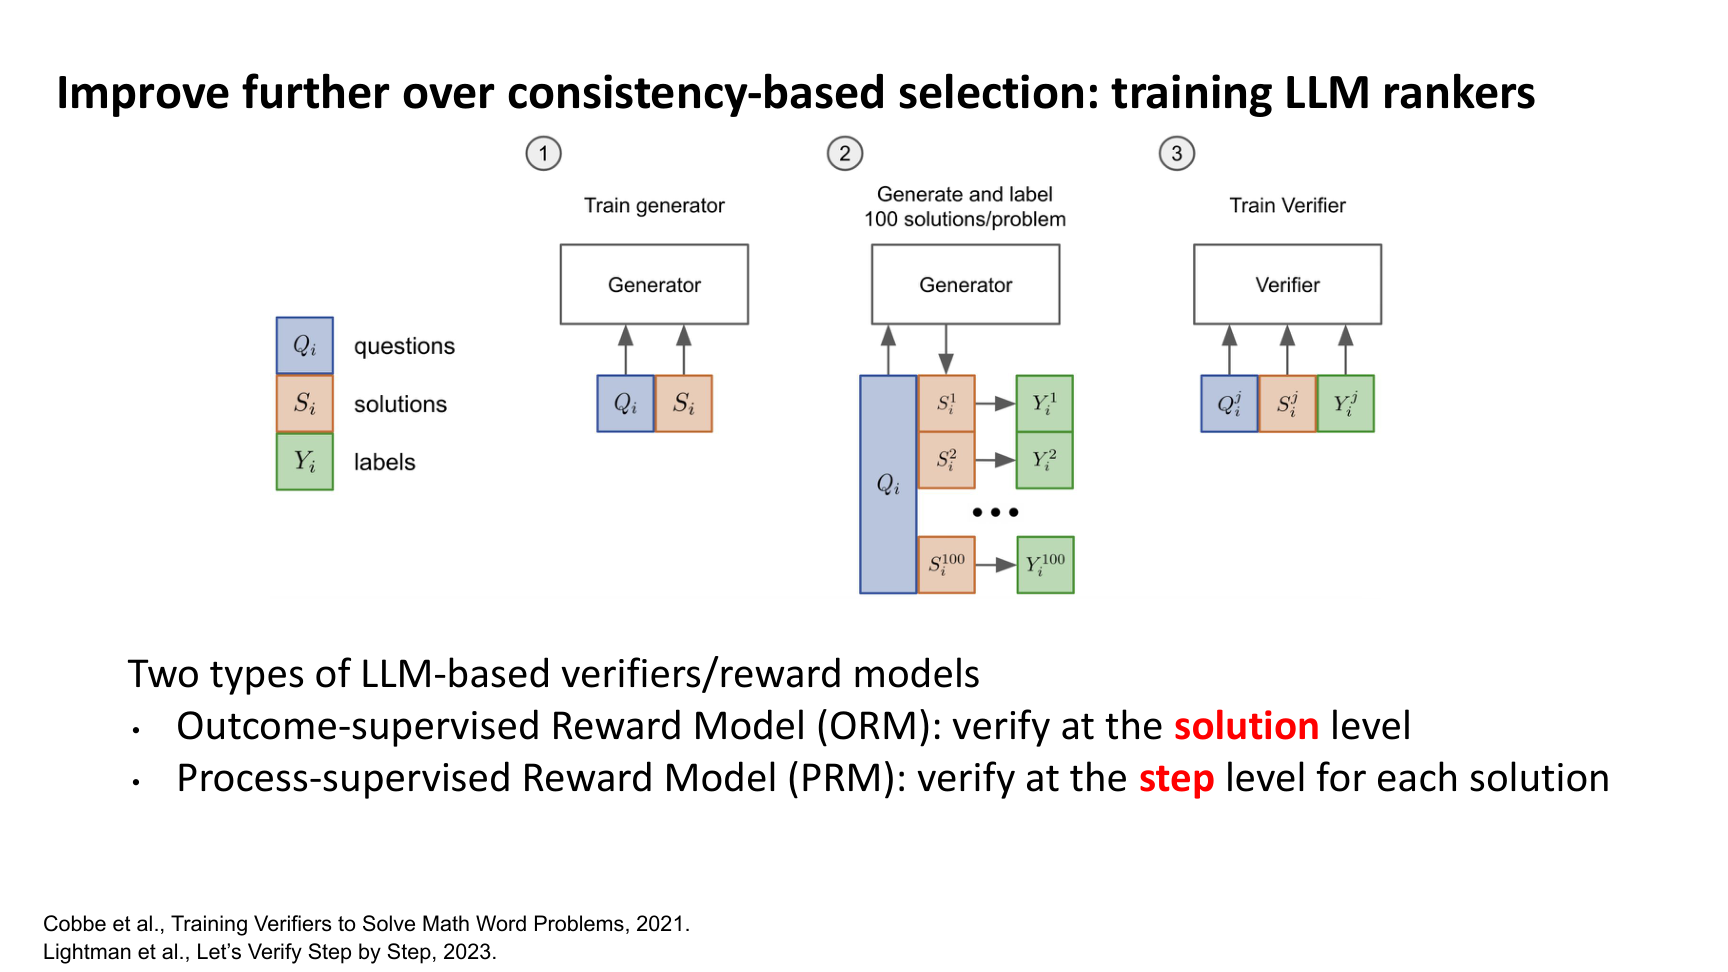
\includegraphics[width=0.75\textwidth]{figures/lec01_fig_010.png}
\caption{Verifier 的两类对象：ORM 在最终结果层面打分，PRM 在中间步骤层面打分。}
\end{figure}

一个统一的抽象写法是：
\[
\tau^{\star} = \arg\max_{\tau \in \mathcal{T}} r_{\phi}(\tau), \qquad
r_{\phi}(\tau)=\sum_{t} r_{\phi}(s_t, a_t)
\]
其中，$\tau$ 表示一条完整或部分 reasoning trajectory，$\mathcal{T}$ 是候选轨迹集合，$r_{\phi}$ 是 verifier 或 reward model 的打分函数，$(s_t,a_t)$ 是第 $t$ 步的状态与动作（或推理步）。

这里有两种不同思想：
\begin{itemize}
\item \textbf{ORM}：对完整答案打一个总分，适合“结果清楚可比较”的任务。
\item \textbf{PRM}：对中间步骤逐步打分，适合“过程质量本身就重要”的任务，如数学推理或程序构造。
\end{itemize}

\paragraph{为什么 verifier 能比 simple voting 更强}
投票只知道“哪些终点重复出现得多”，而 verifier 试图利用更丰富的信息，例如步骤合法性、中间状态质量、与题意的匹配程度。只要 verifier 足够可靠，它就能在“正确答案尚未大量重复出现”之前优先挑出更有潜力的轨迹。

\subsubsection{Tree of Thoughts：在部分解空间上搜索}

Lecture 对 Tree of Thoughts（ToT）的强调在于：前面的方法大多是“先生成完整答案，再筛选”，ToT 则在\textbf{部分思路}层面进行显式搜索。它允许系统生成候选 thought，给部分状态打分，然后决定继续展开哪些分支。

\begin{figure}[H]
\centering
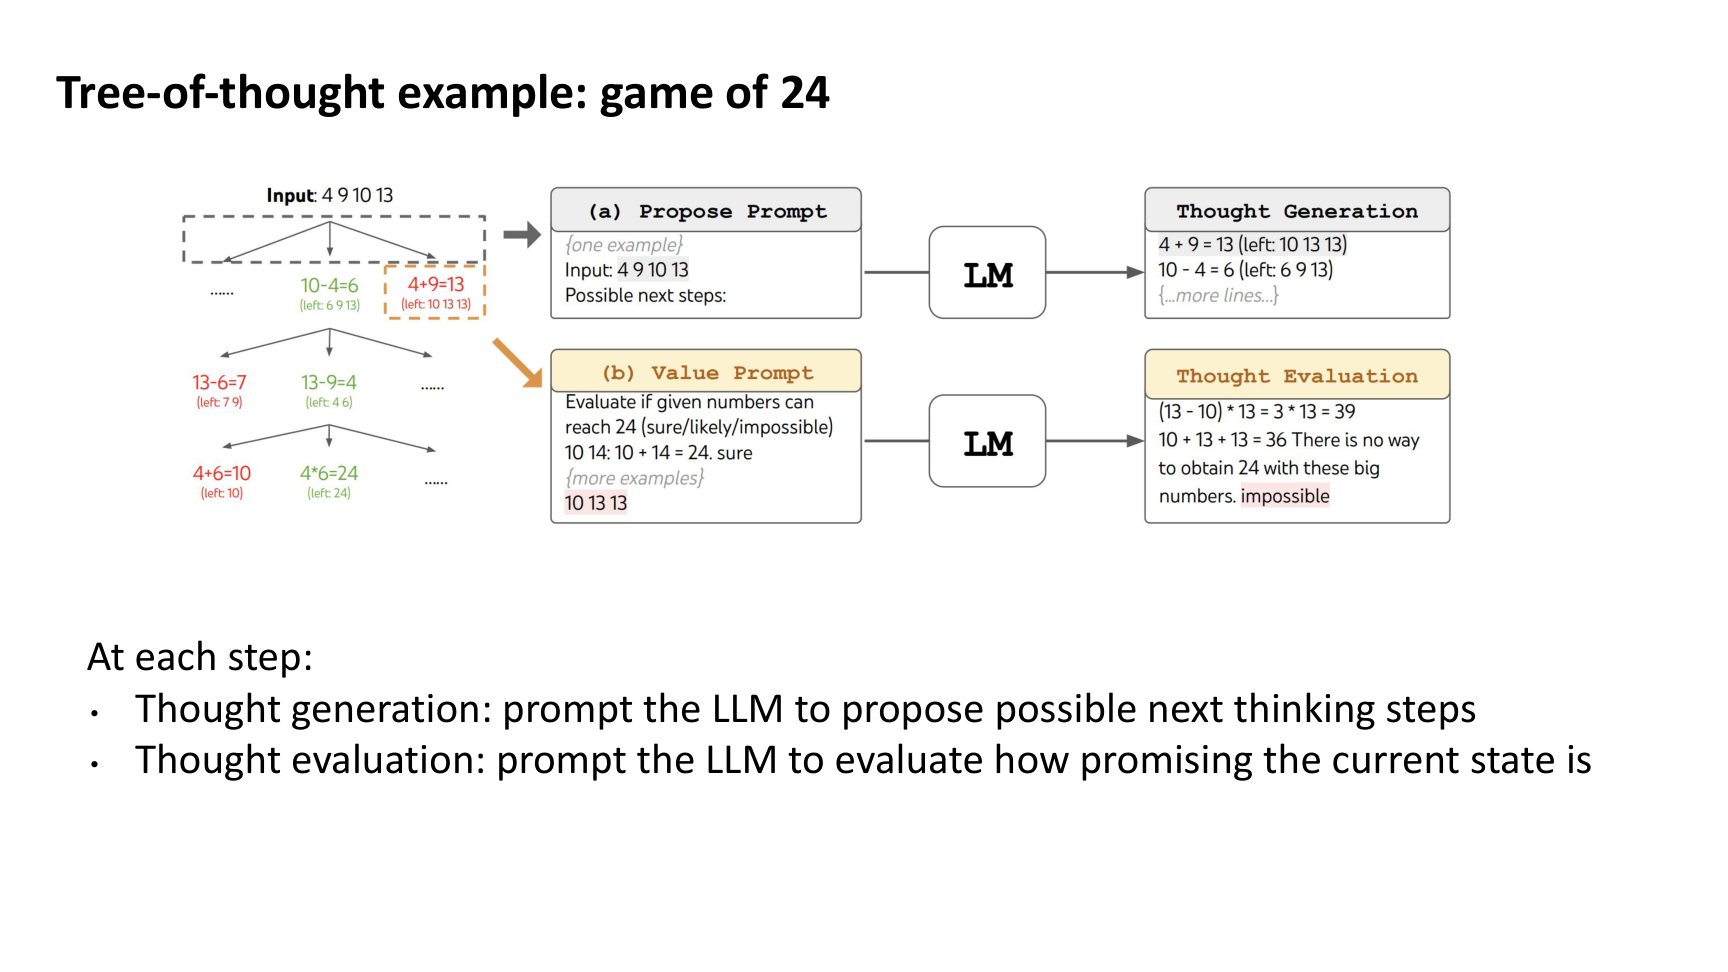
\includegraphics[width=0.74\textwidth]{figures/lec01_fig_011.png}
\caption{Tree of Thoughts 的代表性图：在 partial states 上进行展开和评估，而不是等完整答案生成完再统一筛选。}
\end{figure}

\begin{lstlisting}
Initialize frontier with the empty state
repeat:
    expand candidate next thoughts
    score partial states
    keep the best frontier states
until a complete solution is found or budget is exhausted
\end{lstlisting}

这类算法的优势是：如果某条路径在中途已经显露出坏迹象，系统可以提前剪枝，而不是把预算浪费在完整生成上。它特别适用于\textbf{中间状态可评价}的问题，如 Game of 24、数学证明搜索、程序构造等。

\paragraph{复杂度直觉}
ToT 的难点在于分支爆炸。若每一步都扩展太多 thoughts，而状态评分器又不够准，就会迅速耗尽预算。因此 ToT 不是“越树状越好”，而是要求生成器、评价器和预算控制共同协调。

\subsection{深度自改进：Reflexion、Self-Refine 与 Self-Debugging}

\subsubsection{Reflexion 与 Self-Refine}

Reflexion、Self-Refine 这类方法把重点从“并行多路径搜索”转向“串行修正”。它们的共同模板是：先生成一个答案，再根据反馈写出反思或改进意见，然后基于这些意见重新生成。

它们解决的问题是：有些任务不需要同时探索很多路径，而更需要在已有路径上\textbf{定位错误并迭代修补}。这在长文本写作、计划修正、部分程序修复等场景下很自然。

但 Lecture 明确指出：这类方法只有在\textbf{反馈足够好}时才真正有效。否则模型的“反思”只是在原始错误轨迹附近做风格化改写。

\subsubsection{Self-Debugging：代码领域中的正例}

代码生成是 Lecture 给出的最强正例之一。原因并不是代码比自然语言更容易，而是代码常常有外部信号：测试结果、编译器报错、execution trace、静态分析输出等。这些信号让“修正”不再是空想，而是以客观反馈为依据。

\begin{figure}[H]
\centering
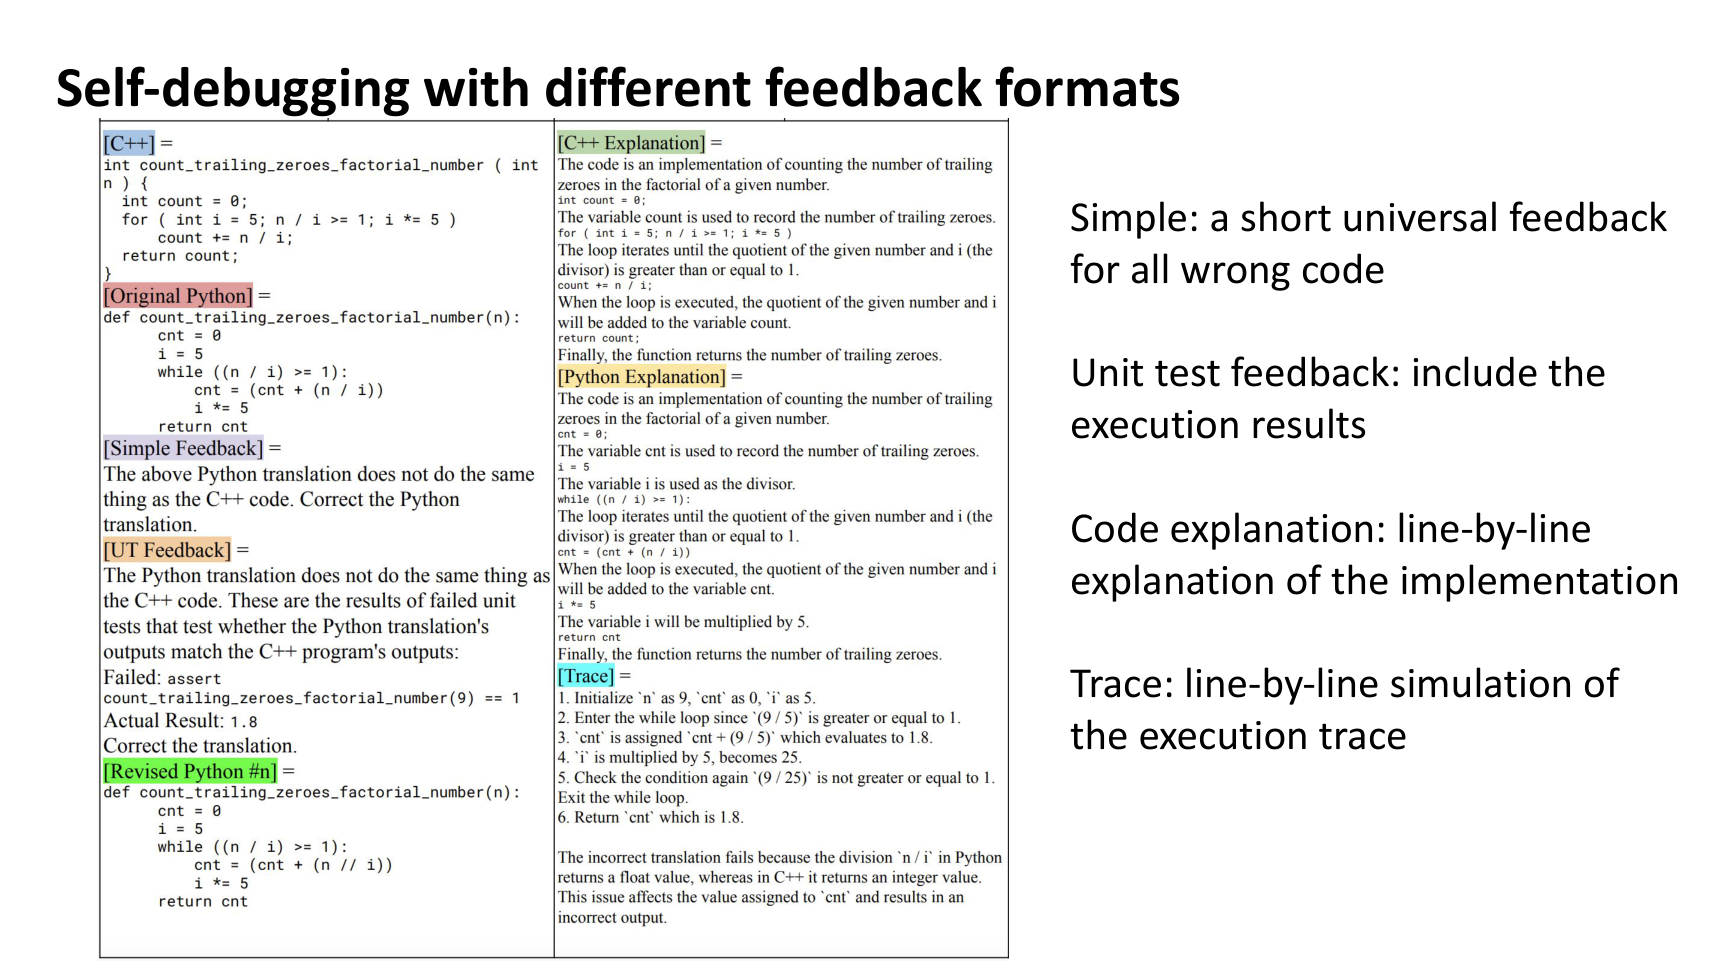
\includegraphics[width=0.72\textwidth]{figures/lec01_fig_012.png}
\caption{Self-Debugging 在代码任务中的反馈形态：从简短反馈到 execution trace，信息密度越来越高。}
\end{figure}

\begin{lstlisting}
Generate code
Run tests or inspect execution results
Ask the model to explain/debug the program
Revise the code using the observed feedback
\end{lstlisting}

\paragraph{为什么这不是“单纯多试几次”}
Self-Debugging 的本质不是重复采样，而是把\textbf{失败信息回流到生成过程}。执行结果告诉模型哪条路径错了，代码解释迫使模型定位错误机制，修订步骤则把反馈转化成新的程序候选。

\paragraph{Reading 连接}
\emph{Teaching Large Language Models to Self-Debug} 表明，在 Spider、TransCoder、MBPP 等任务上，只要能提供执行反馈或解释过程，模型就能显著提升代码质量。这个 reading 在本讲中的作用是证明：\textbf{自改进不是幻想，但它依赖可信外部信号。}

\subsection{为什么很多 Self-Correction 会失败}

这一节是本讲最重要的反直觉结论之一。直觉上，人们容易以为“既然 LLM 会反思，那就让它自己看看自己的答案，再改一遍”。但 \emph{Large Language Models Cannot Self-Correct Reasoning Yet} 和 lecture 中的实验结果表明：\textbf{如果没有 oracle 或任务接近真实目标的外部反馈，self-correction 往往不但不稳定，甚至可能更差。}

\begin{figure}[H]
\centering
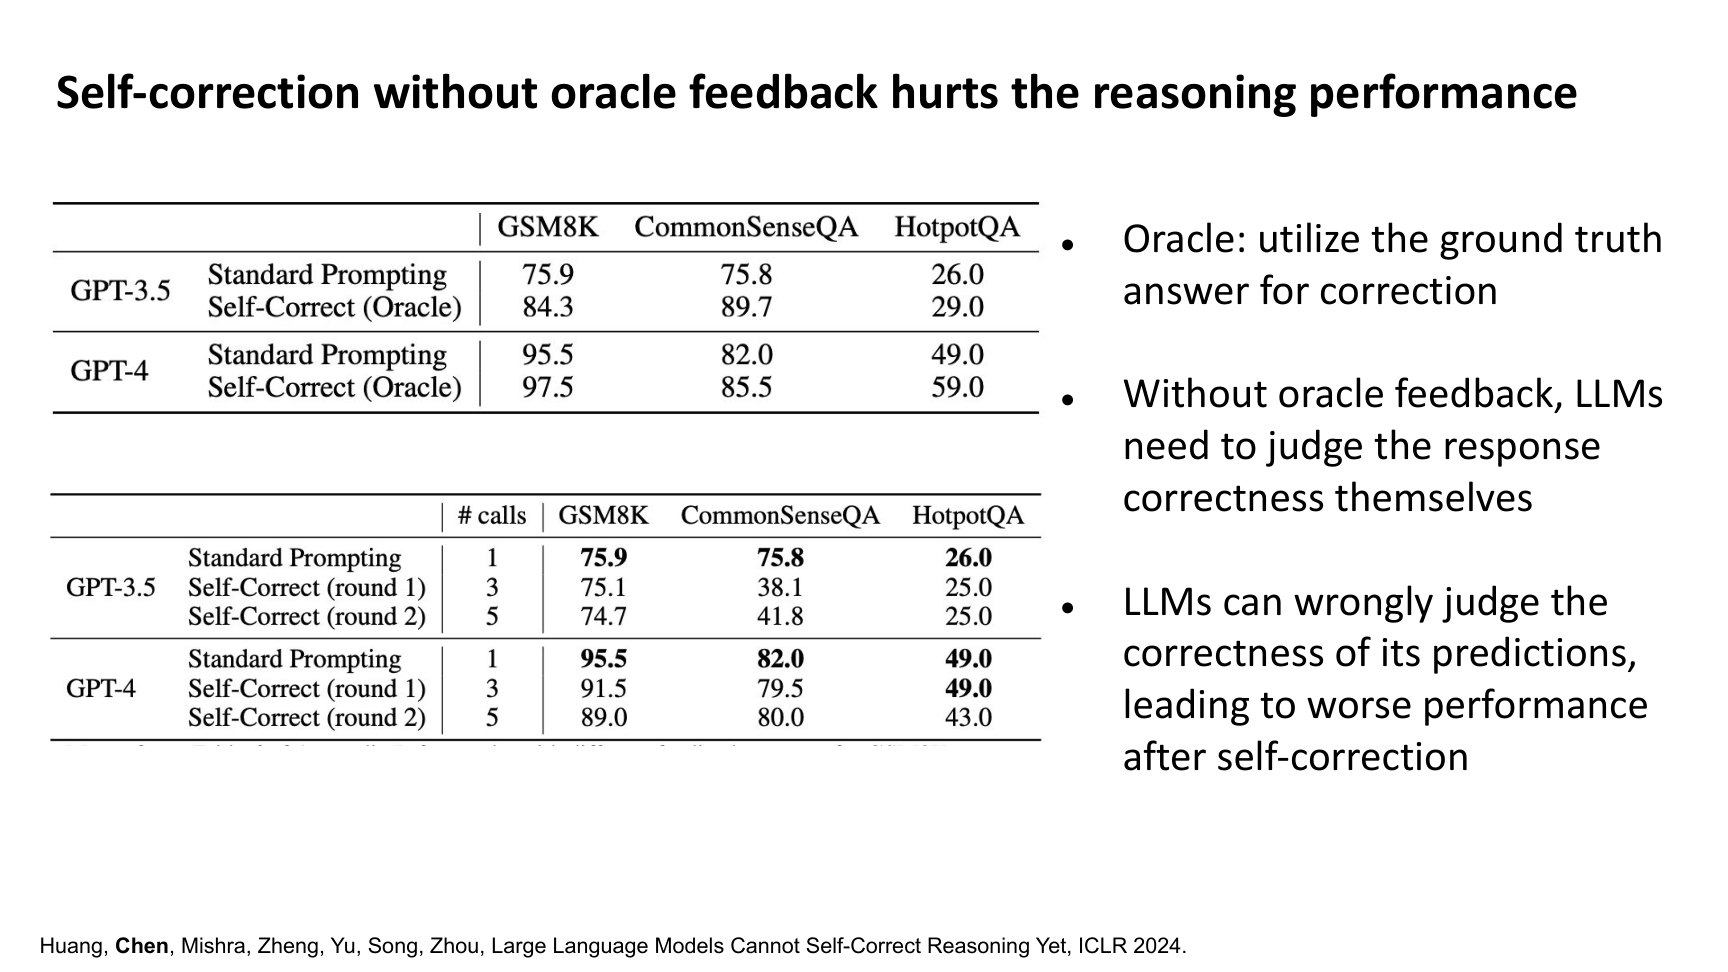
\includegraphics[width=0.72\textwidth]{figures/lec01_fig_013.png}
\caption{Lecture 的负面结果页：对 QA-style reasoning 任务，没有可靠外部反馈时，self-correction 可能降低性能。}
\end{figure}

原因在于，模型的“第二次思考”并不会天然比第一次更接近真值。它可能：
\begin{itemize}
\item 只是把原有错误换一种说法重复一遍。
\item 受到表面流畅性的诱导，修改成更自信但更错的答案。
\item 过度相信自己构造的伪反馈，从而偏离真实目标。
\end{itemize}

Lecture 还指出，多 agent debate 也不能自动解决这一问题。如果每个 agent 共享同类偏差，而又缺少真正独立的外部检验，那么“辩论”只是在更大系统里复制同样的错误。

\begin{warningbox}{一条必须记住的原则}
自我修订只有在\textbf{评价器足够可信}时才值得花额外算力。没有外部反馈时，把预算砸在多轮自我说服上，常常不如把预算花在更宽的采样或更强的 verifier 上。
\end{warningbox}

\subsection{推理时预算分配：宽度、深度、模型规模}

Lecture 最后把前面的技术统一到一个预算分配问题上：
\[
\max_{M,N,D} \ \operatorname{Acc}(M,N,D)
\quad \text{s.t.} \quad C(M,N,D) \le B
\]
这里，$M$ 表示模型规模或模型家族选择，$N$ 表示并行采样宽度，$D$ 表示串行修正或搜索深度，$C$ 是总推理成本，$B$ 是给定的预算。

\begin{figure}[H]
\centering
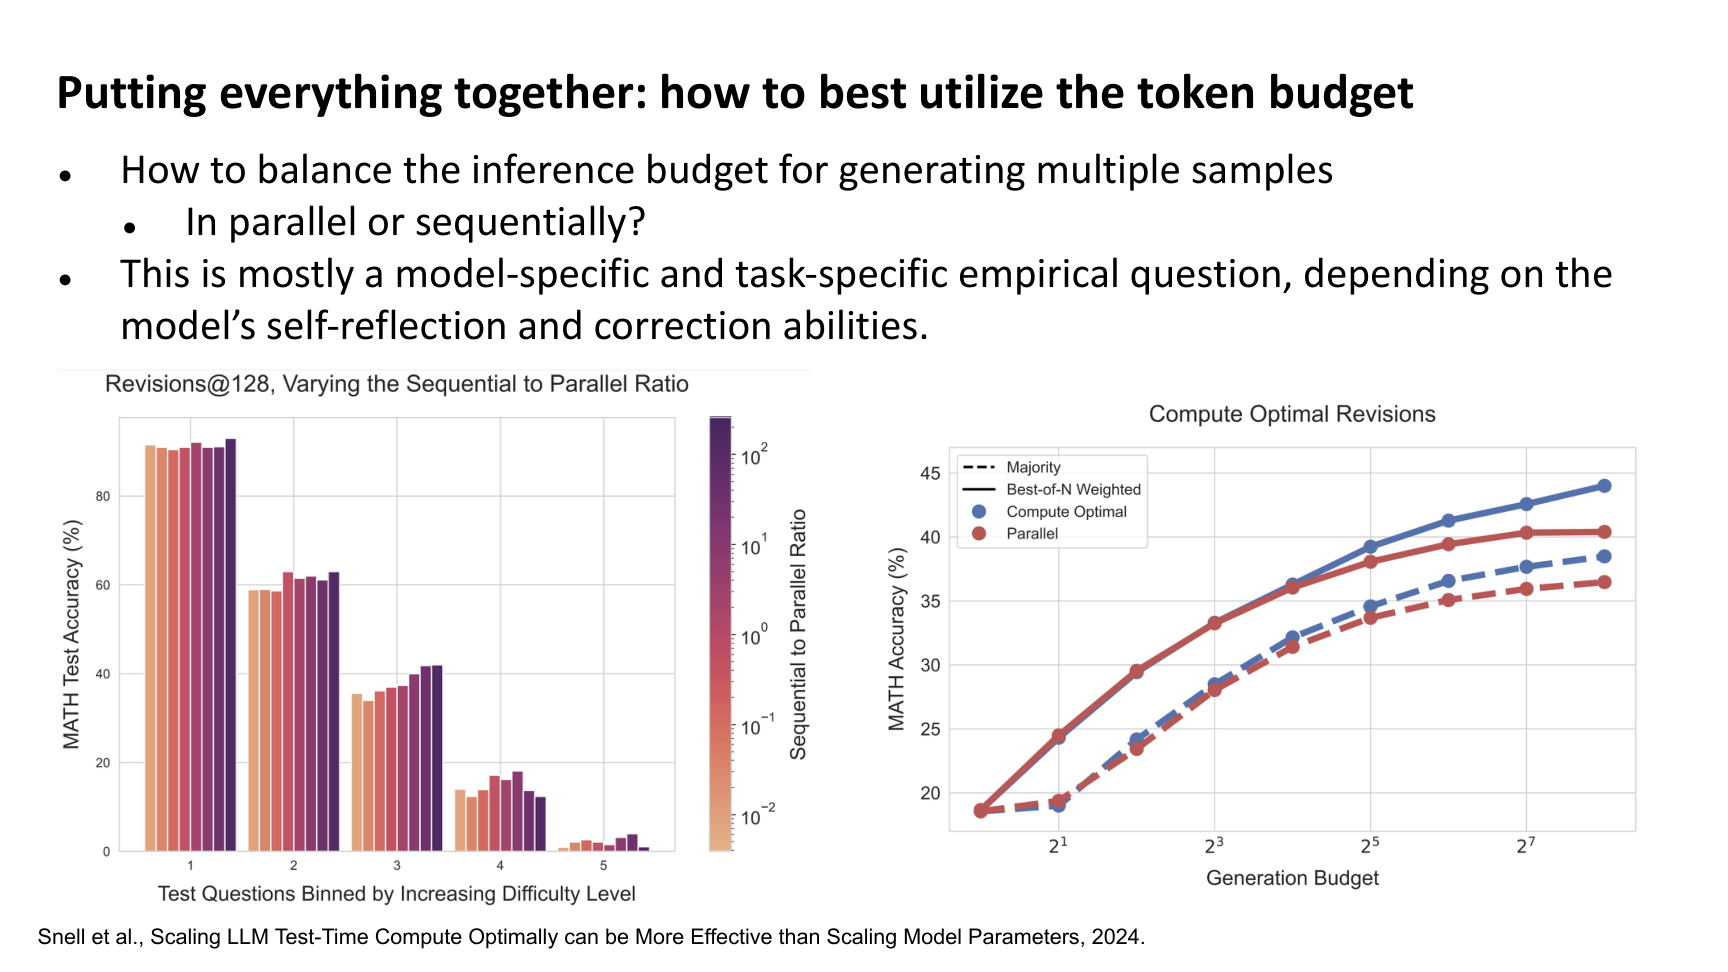
\includegraphics[width=0.74\textwidth]{figures/lec01_fig_014.png}
\caption{推理时预算分配问题：并行采样、串行修正、评分器调用和模型规模选择，都会消耗 test-time budget。}
\end{figure}

这条公式的意义不在于给出闭式解，而在于告诉我们：\textbf{“多想一点”不是单一变量。} 你可以把预算花在：
\begin{itemize}
\item 更大的模型上；
\item 更多并行样本上；
\item 更深的修正循环上；
\item 更强的 verifier 调用上；
\item 更复杂的搜索树上。
\end{itemize}

不同任务的最优分配并不相同。数学推理可能更依赖步骤级 verifier；代码问题可能更依赖执行反馈；开放式问答则可能更适合宽采样配合较弱筛选。

\subsection{Bitter Lesson 在本讲中的含义}

Lecture 最后一页把所有方法上升到一个一般设计原则：当我们设计 reasoning technique 时，应优先押注那些\textbf{随着计算量增加仍能继续扩展的通用方法}，而不是严重依赖人手雕刻规则的脆弱技巧。

\begin{figure}[H]
\centering
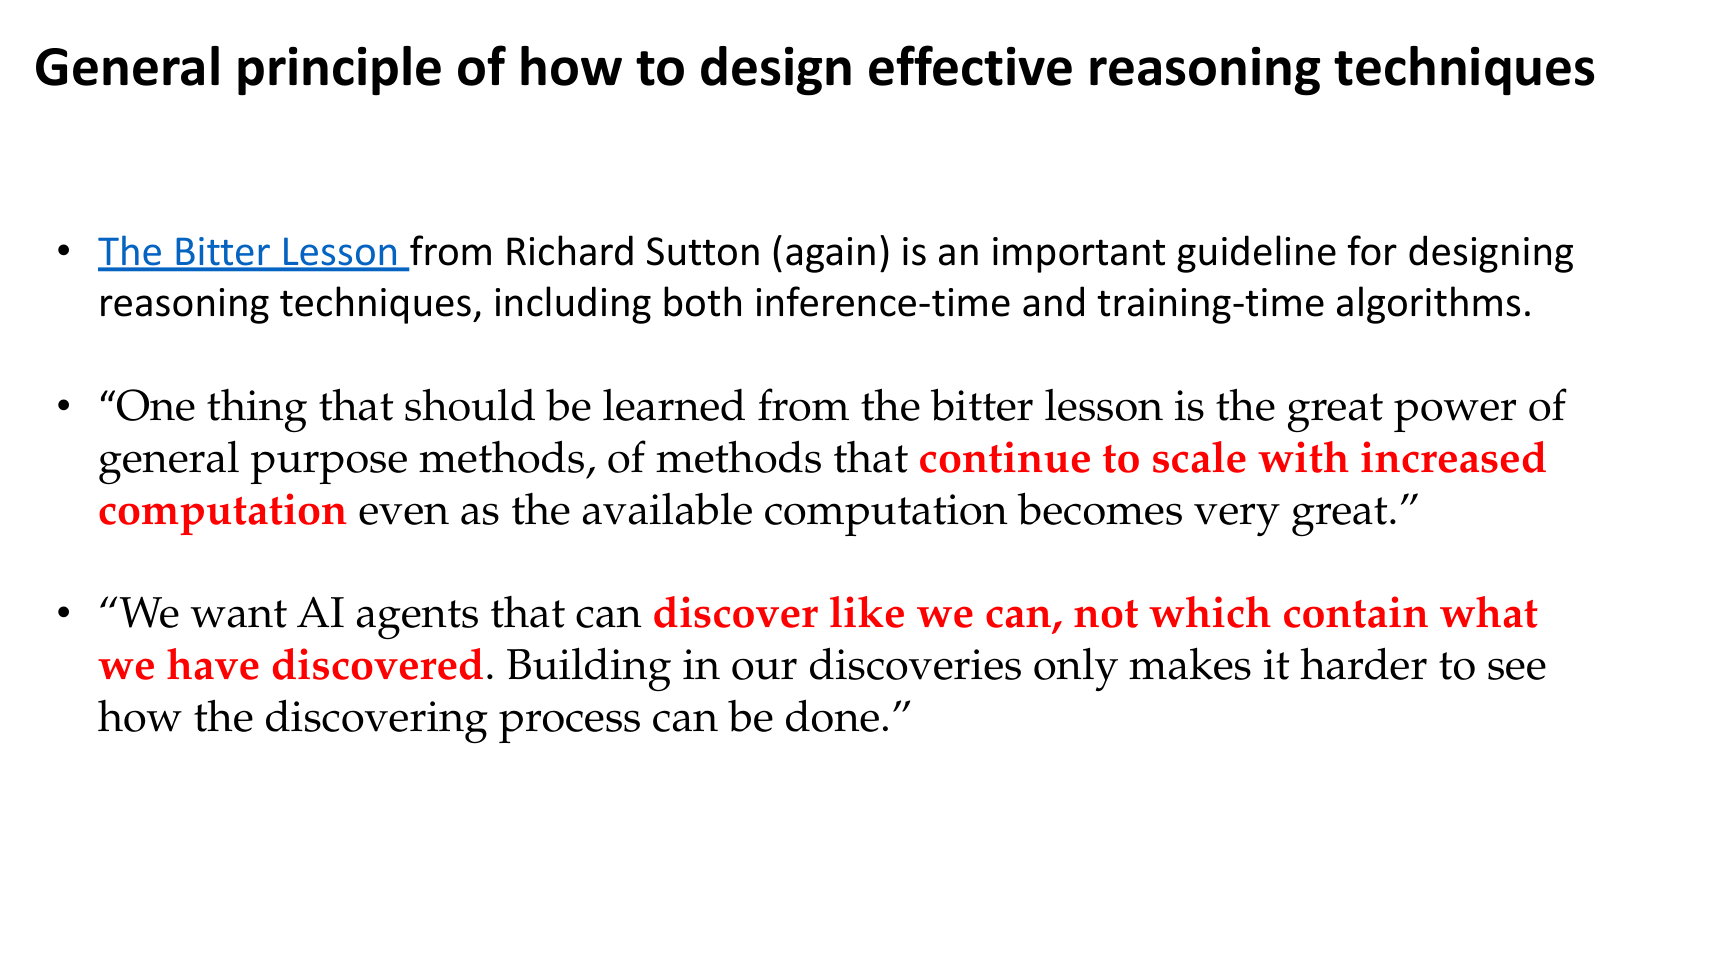
\includegraphics[width=0.72\textwidth]{figures/lec01_fig_015.png}
\caption{本讲的设计原则：偏好那些随计算增长而持续扩展的通用 reasoning 方法。}
\end{figure}

这就是本讲对 Bitter Lesson 的重新解释。它并不是说“永远不要做结构设计”，而是说：好的结构设计应当服务于\textbf{可扩展的搜索、评价与修正机制}，而不是把性能寄托在难以泛化的手工小技巧上。

\section{关键论文与课程 readings 的连接}

\subsection{Large Language Models as Optimizers}

这篇论文的核心贡献不是“找到了一种更好的 prompt”，而是把 prompt search 明确化。它问的是：既然候选 prompt 可以被打分，为什么不能让 LLM 自己观察历史候选及其得分，然后继续提出新候选？ 这直接对应 lecture 在 OPRO 那部分的思想。对于 LLM agents 来说，这意味着\textbf{语言模型不仅可以当策略，还可以在推理时兼任局部优化器。}

\subsection{Large Language Models Cannot Self-Correct Reasoning Yet}

这篇论文在本讲中承担“刹车片”的角色。它提醒我们：self-correction 不是白送的推理增益。没有可靠反馈时，额外轮次并不等于更强 reasoning。对 agent 系统而言，这意味着任何“让 agent 自己检查自己”的流程，都必须仔细审查反馈源是否真的和任务目标一致。

\subsection{Teaching Large Language Models to Self-Debug}

这篇论文给出了反例：在代码任务上，自我改进确实能奏效，因为程序拥有可执行的外部环境。测试、trace 和错误信息把反馈从“感觉上应该不对”变成了“这里具体不通过”。它是 lecture 中“为什么代码任务是 agent workflow 天然试验场”的最好说明。

\section{例子、反例、失败模式和边界条件}

\subsection{一个统一对比：同样的预算，花在哪最有效}

假设你有固定 budget。你可以：
\begin{itemize}
\item 用一个较大模型只采样一条答案；
\item 用中等模型采样十条 CoT，然后 Self-Consistency；
\item 用中等模型采样五条，再让 verifier 排序；
\item 用较小模型跑多轮 self-refine；
\item 对代码问题把 budget 主要花在执行与修复循环上。
\end{itemize}

本讲的关键结论不是哪一种永远最好，而是：\textbf{要看任务是否拥有外部反馈、是否能给中间状态打分、以及错误是“路径选错”还是“局部算错”。}

\subsection{常见失败模式}

\begin{enumerate}
\item \textbf{把更长 CoT 误认为更好 reasoning。} 如果中间步骤不受任何约束，只会产生更长的幻觉。
\item \textbf{把多样采样误认为真正搜索。} 若样本高度同质，Self-Consistency 不会带来宽度增益。
\item \textbf{把 LLM judge 当成可靠 verifier。} 如果 judge 没有额外 grounding，它只是把原模型偏差迁移到了选择阶段。
\item \textbf{在没有外部反馈时过度依赖 self-correction。} 这在 QA-style reasoning 上尤为危险。
\item \textbf{忽略成本。} 某些方法虽然能提分，但在 wall-clock、API cost 或 latency 上不可接受。
\end{enumerate}

\subsection{与前后讲的联系}

本讲主要处理\textbf{推理时}如何使用计算与反馈。下一讲“Learning to reason with LLMs”则会把问题转向\textbf{训练时}如何通过偏好优化、过程监督或后训练让模型更擅长 reasoning。换句话说，本讲问“同一个模型如何在 deployment 时更聪明地使用算力”，后续讲次会问“如何让模型本身更容易被教会这些行为”。

\section{总结与延伸}

第一讲的最大价值，在于给整门课建立了一个统一视角：\textbf{Advanced LLM agents 的很多能力，都是通过对推理轨迹的生成、选择、评价和修正来实现的。} CoT、Analogical Prompting、OPRO、Self-Consistency、Verifier、Tree of Thoughts、Self-Debugging 看起来不同，但它们都在重新分配 inference-time budget，并试图让额外计算真正转化成更高质量的 reasoning path。

如果把本讲压缩成一句话，那就是：

\begin{center}
\emph{不要只问模型“会不会”，还要问系统“如何在推理时把计算花在最有价值的地方”。}
\end{center}

\subsection{本章小结}

\begin{itemize}
\item CoT 系列方法的价值在于显式暴露中间推理，而不只是追求更长回答。
\item Analogical Prompting、Least-to-Most 和 Self-Discover 说明：推理结构本身也是 inference-time 可优化对象。
\item Self-Consistency、verifier、ToT 把“多生成一些”升级成“有选择地搜索和筛选”。
\item Self-Debugging 之所以有效，关键不在“反思”二字，而在于外部可执行反馈。
\item 没有可靠反馈时，self-correction 往往不值得额外预算。
\item 设计 reasoning technique 时，应优先考虑那些可随计算量增加而扩展的方法。
\end{itemize}

\section{复习题}

\begin{enumerate}
\item 为什么说 Standard Prompting 的问题不只是“提示词不够好”，而是没有显式给中间推理分配预算？
\item Few-shot CoT 与 Zero-shot CoT 的主要差别是什么？它们分别在哪些场景更有优势？
\item Analogical Prompting 的两个阶段各自起什么作用？
\item OPRO 为什么可以被理解为 inference-time optimization，而不只是 prompt tweaking？
\item Self-Consistency 与 beam search 的差别在哪里？
\end{enumerate}

\section{深入思考题}

\begin{enumerate}
\item 如果某个任务没有明确的最终答案抽取器，你会如何设计 Self-Consistency 的聚合机制？
\item 在什么条件下，PRM 会明显优于 ORM？请结合数学推理或程序合成举例说明。
\item 设想一个没有外部执行环境的开放式写作任务。你会如何构造“足够可信”的反馈，使自我修订不至于退化成自我说服？
\end{enumerate}

\section{实践题与延伸阅读}

\begin{itemize}
\item 实践题：实现一个最小版 Self-Consistency 解码器，在同一题目上采样 $N$ 条 CoT，并比较不同温度和不同 $N$ 的答案聚合效果。
\item 实践题：把 OPRO 的优化循环实现为一个 prompt-search harness，观察 instruction 历史如何影响下一轮候选。
\item 阅读延伸：进一步阅读 \emph{Tree of Thoughts}, \emph{Let's Verify Step by Step}, \emph{Scaling LLM Test-Time Compute Optimally can be More Effective than Scaling Model Parameters}，并思考这些工作如何共同描述一个“预算受限的 reasoning system”。
\end{itemize}

\end{document}
